\section{Struktura Aplikace}

Aplikace je tvořena jediným oknem a systémovými upozorněními. Pokud uživatel chce pracovat na více projektech zároveň, může si Aplikaci na jednom počítačí otevřít několikrát naráz.


\begin{figure}[ht]
	\centering
	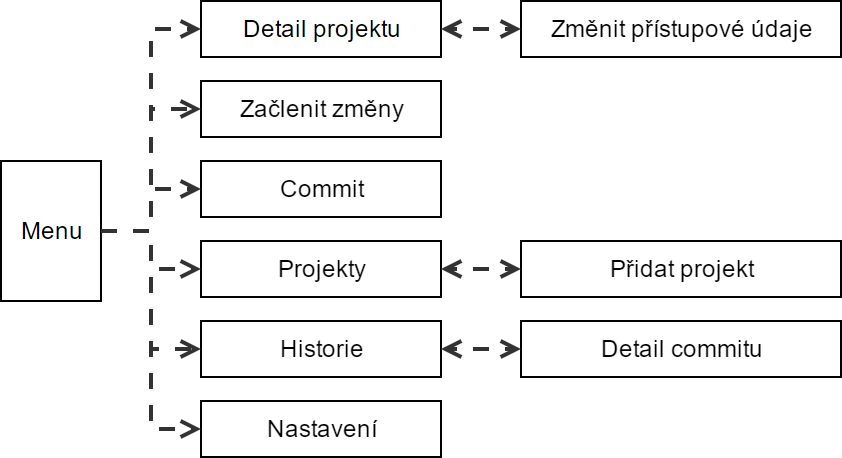
\includegraphics[width=\textwidth]{sections/ui/images/flow.png}
	\caption{Diagram struktury uživatelského rozhraní}
\end{figure}

Po levé straně se nabízí rozbalovací menu, jež může obsahovat položky detail projektu, „Commit“, „Projekty“, „Historie“ a „Nastavení“. První zmíněná položka je nahrazena názvem projektu. Vstupní obrazovkou je stránka s projekty, která se také zobrazuje vždy po spuštení aplikace. Obsahuje seznam projektů, které si uživatel do Aplikace přidal pomocí tlačítka plus (Floating Action Button) v pravé dolní části této obrazovky. U každého projektu v seznamu se zobrazuje zvýrazněný název adresáře a jeho celá cesta v lokálním souborovém systému. Dále dvě tlačítka, „ZVOLIT“ a „ODEBRAT“, případně „DETAIL“ a „ODEBRAT“, kde zvolením nastaví uživatel konkrétní projekt jako aktivní, což je ten, na kterém hodlá pracovat. Tlačítkem pro detail je uživatel přesunut na obrazovku s detailem projektu a odebráním dojde k vymázání projektu ze seznamu projektů, nedojde však k úplnému smazání ze souborového systému, takže uživatel může kdykoliv projekt přidat zase zpět. Název aktivního projektu se zobrazuje v horním App baru.

% @TODO: Snackbar
Tlačítkem pro přidání projektu se otevře modální okno obsahující volbu mezi přidáním z adresáře či z URL. První možnost dává na výběr z adresářů na lokálním počítači, u kterých se očekává, že budou obsahovat již existující projekt propojený s Gitem. Při přidávání z URL se zadává adresa repozitáře, v Gitu označováno jako „remote“ a prázdný adresář, do kterého se projekt stáhne, terminologií Gitu naklonuje. Úspěchy a neúspěchy během těchto a jim podobných procesů jsou ohlašovány pomocí komponenty Snackbar, která v takových situacích vyjíždí z dolní části okna s krátkou zprávou či natlačítkem například pro zrušení akce, která vedla k tomuto zobrazení. Snackbar vyjíždí na tři sekundy třeba po úspěšném přidání projektu do seznamu.

% @TODO: Gravatar
Obrazovka detailu projektu prezentuje přehled o aktivním projektu. Odkaz v menu mizí, pokud není žádný projekt zrovna aktivní. Přehled se dělí až na čtyři sekce v závislosti na vlastnostech projektu. V první části se zobrazují autoři. Každý autor má avatara, který je poskytnut službou Gravatar, jenž nabízí volně dostupné obrázky, které si uživatel může připojit ke své e-mailové adrese, jméno, e-mail a čas, kdy naposledy prováděl v projektu úpravy. Čas je relativní k aktuálním okamžiku a průběžně se aktualizuje. Druhá část obsahuje odkaz na již zmíněný remote, který lze využít v případě sdílení projektu s dalšími autory. Součástí projektového detailu je také stručná analýza běžného commitu. Ta vychází z mediánů přianých řádků, odebraných řádků a změněných souborů ve všech commitech. Tyto hodnoty se využívají pro doporučování vhodného času pro vytvoření nového commitu. Poslední část nabízí změnu přístupových údajů a zobrazuje se jen u projektů, jejichž remote začíná na „http“, protože právě u takových projektů může být vyžadováno uživatelské jméno a heslo. Tlačítkem „ZMĚNIT“ se otevře modální okno s formulářem právě na tyto dvě položky předvyplněné posledními známými hodnotami.

% @TODO: ukázka notifikace
V případě, že uživatel provedl v aktivním projektu nové změny, které nejsou zatím commitnuté, v menu se zobrazí položka „Commit“. Pokud změny překročí minimálně dvě ze tří charakteristik běžného commitu, uživatel dostane systémové upozornění, které po rozkliknutí přenese do popředí okno Aplikace a zobrazí patřičnou obrazovku. S příchodem upozornění se i v Aplikaci rozsvítí v levém horním rohu a v menu (Drawer) vykřičník, který zmizí po zobrazení obrazovky pro vytvoření commitu. Na této obrazovce jsou tlačítka označit/odoznačit vše a aktualizovat. Aktualizováním se znovu načte seznam pozměněných souborů, které jsou zvolené pro začlenění do nového commitu a seznam souborů, které jsou sice také nově přidané, změněné či nově odstraněné, ale nebudou do commitu zahrnuté. Pod seznamy je textové pole pro stručný popis změn, tlačítko pro uložení, které vytvoří commit a náhled zvolených změn.

Náhled změn obsahuje názvy souborů, které se změnily s popiskem, o jakou změnu se jedná. V popisku se tak často objevuje například informace, že soubor byl nově vytvořen, upraven, přejmenován či odstraněn. Pokud se jedná o textový soubor se změněným obsahem, je popis doplněn i o seznam přidaných a odebraných řádků. Řádky jsou označené čísly, jež reprezentují číslo řádku před či po změně v souboru, znaménkém, kde plus symbolizuje nový řádek a minus pro odebraný, stejně tak zelené pozadí pro nový a červené pro odebraný, a doplněné samotným obsahem řádku.

Každý projekt má přehled historie, což jen jednosloupcový či dvousloupcový seznam commitů na hlavní větvi. V levém sloupci se zobrazují commity, které jsou nahrané na vzdáleném serveru, případně jejich poslední stav před ztrátou spojení se vzdáleným serverem. Commity, které jsou zvýrazněné pouze červenou barvou, nejsou promítnuté do souborů, na nichž uživatel aktuálně pracuje. V pravém sloupci se zobrazují commity, které zatím nejsou nahrané na vzdálený server a nejsou tudíž zazálohované a sdílené s ostatními autory. Nejnovější se zobrazují nejvýše. Délka historie je omezena na 250 položek, protože při vyšších počtech ztrácí Aplikace rychlou odezvu. Kliknutím na libovolný commit lze zobrazit jeho detail. Tento detail je hodně podobný náhledu při vytváření commitu. Je akorát navíc doplněn unikátním identifikátorem commitu, informací o autorovi s časem vytvoření a tlačítkem pro rychlý návrat na přehled historie.

Pokud některý z ostatních autorů nasdílí nové změny, aplikace zobrazí systémové upozornění nehledě na to, zdali je hlavní okno v popředí. Upozornění obsahuje stručnou informaci, že jsou k dispozici nové změny a po rozkliknutí přesune uživatele do Aplikace s obrazovkou pro začlenění změn.

Při začleňování změn má uživatel k dispozici dvě tlačítka a seznam všech známých nezačleněných změn v již známém stylu z vytváření commitu a z detailu commitu. První tlačítko je zvýrazněné a slouží pro přijetí změn, což provede sloučení větve lokální se vzdálenou. Druhé tlačítko aktualizuje seznam upravených souborů.

Poslední obrazovkou, která je v menu vždy dostupná, je nastavení. Zde učivatel může volit mezi českým a anglickým jazykem uživatelského rozhraní, vypnout či zapnout automatické sdílení lokálních změn a obnovit tyto dvě položko do původního stavu jako po prvním spuštění, což nastavý český jazyk a povolí automatické sdílení.
